\chapter{Background}
\section{Definition of terms}
To prevent missunderstandings and confusion, the following subsections 2.1.1 - 2.1.x will define some terminoligy which will be mandatory for the understanding of certain areas of this thesis.

\subsection{Deep Zoom Image Format}
The Deep Zoom Image Format (.dzi)\nomenclature{.dzi}{Deep Zoom Image Format} is an xml-based file format maintained by Microsoft to improve performance and quality in the handling of large image files. For this purpose an image is represented in a tiled pyramid (see fig. 2.1).
			
\begin{figure}[!htbp]
	\begin{center}
		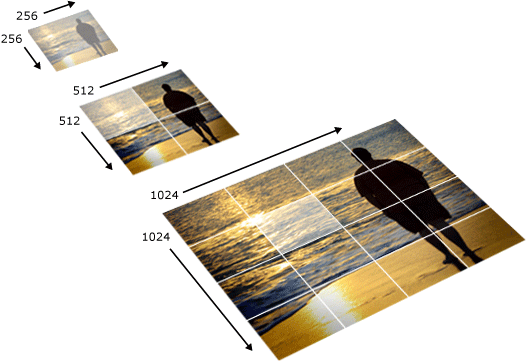
\includegraphics[scale=0.5]{img/dzi_pyramid.png}
		\caption{3 consecutive levels of a .dzi image (source: https://i-msdn.sec.s-msft.com/dynimg/IC141135.png)}
		\label{fig:fig2.1}
	\end{center}
\end{figure}

As seen in fig. 2.1 there are multiple versions of a single image in different resolutions. Each resolution in the pyramid is called a \emph{level}. At each level the image is scaled down by the factor 4 (2 in each dimension). Furthermore, the image gets tiled up into $256^2$ tiles (256 in each dimension)\cite{web:dzi}.

If a viewer wants to view a certain area of the image (e.g. the highlighted tile in the last image in fig. 2.1), only the corresponding tiles need to be loaded. This saves large amounts of bandwidth and memory. The same goes for a viewer, who is zoomed out very far. In such a view the full level of detail isn't needed, so that a version from a lower level can be loaded.

A .dzi file consists of two parts: a describing .xml file\footnote{Frameworks like \emph{OpenSeaDragon} also support further formats, such as .json.} and a folder with more subfolder. Each subfolder describes a level and as such contains all the tiles for that particular level.

%In other words, a level can be defined as an image with the resolution $level^2$ for height and width, resulting in a resolution of $level^4$. Levels are counted from level 0 (1*1 Pixel) \cite{web:dzi}. E.g. the levels shown in fig. 2.1 are:
%\begin{itemize}
%	\item level 8 ($2^8=256$) for the $256^2$ pixel image
%	\item level 9 ($2^9=512$) for the $512^2$ pixel image
%	\item level 10 ($2^{10}=1024$) for the $1024^2$ pixel image
%\end{itemize}


\subsection{Microservice}
\subsection{Machine Learning}
\subsection{Neural Networks}
\section{Process chain}
\subsection{Description}
\subsection{Definition of Conversion Service}
\subsection{Definition of Annotation Service}
\subsection{Definition of Tesselation Service}